\documentclass[10pt, titlepage]{article}

%设置页边距
\usepackage{geometry}
\geometry{left=2.5cm,right=2.5cm,top=2.5cm,bottom=2.5cm}

%地址链接支持
\usepackage{hyperref}

%页眉页脚
\usepackage{fancyhdr}
\pagestyle{fancy}
\lhead{}
\rhead{}



%设置字体
\usepackage{multirow}
\usepackage[no-math]{fontspec}
\usepackage{xunicode}
\usepackage{xltxtra}
\usepackage{amsmath,amssymb, esint}
\usepackage{chemarrow}
\usepackage[indentfirst=false,slantfont,boldfont]{xeCJK}

\makeatletter
\newcommand{\xLeftrightarrow}[2][]{\ext@arrow 3359\Leftrightarrowfill@{#1}{#2}}
\newcommand{\xRightarrow}[2][]{\ext@arrow 3359\Rightarrowfill@{#1}{#2}}
\makeatother


\setCJKmainfont[ItalicFont={Xingkai SC Light}, BoldFont={Songti SC Bold}]{Songti SC Light}
\setCJKsansfont{Lantinghei SC Extralight}
\setCJKmonofont{Songti SC Regular}

%设置换行缩进
\usepackage{indentfirst}

%行距
\linespread{1.2}

\usepackage{multirow}

\usepackage{xcolor}
\usepackage{caption}
\usepackage{float}
\usepackage{longtable}

\begin{document}

\title{
\Huge\textbf{多模态的社交表情动态植入}
% \\\large{Tsinghua University, Beijing, China}
% \\\large{Natural Language Processing Lab, Department of Computer Science and Technology}
}


\author{
韩旭\thanks{\href{mailto:计33 2013011343}{计33 2013011343}}\quad
赵珮君\thanks{\href{mailto:助教}{助教}}}

\date{2016年7月}
\maketitle
\renewcommand{\contentsname}{\textbf{Contents}}
\renewcommand{\figurename}{\textbf{figure}}
\renewcommand{\tablename}{\textbf{table}}
\tableofcontents
\newpage



\section{概述}
表情是当今社交平台中人与人之间交流的重要组成部分,无论是线上的亦或是线下的。这种随着社交平台兴起的表述方式,通过其自身类人的图案将一些复杂并意味深长的情绪表述蕴藏其中,从而在交流中更为有效。并且从以往的研究来看,在社交平台的交流上,表情是一种有效概括、表述、传达信息的描述形式,并且广泛存在在各个不同文化的国家中,具有普适性。但不同文化、种群之间,不同社交平台和交互设备之间,表情所表述的具体含义又有一定的区别,又具有差异性。由此而来,让机器根据人的社交信息去平滑的构建表情,从而克服这种普适性和差异性之间的矛盾就变的十分有趣。得益于最近在机器学习和多媒体处理技术的发展,这种自动的对社交文字和媒体信息进行反馈的想法可以得到实现,并且在情感分析上已经有了很优秀的成果。但极少有模型将表情纳入到这体系之中。在我们的这篇工作里,我们提出了一套测试基准和实现模型,能够很好的让机器将表情生成到文本和其他媒体上。我们基于LSTM序列模型构建了整体框架,并且充分考虑到社交平台中多模态的特性,将文字和图片同时纳入进来,从而得到一个信息丰富的网络为我们的工作服务。为了体现不同文化和平台的差异性,我们用同样的模型在中文的微博以及英文的Twitter上进行了测试(最大的中文微博平台和应用范围最广的英文社交应用)。实验表明,模型在两种主流的语言上均有很好的表现,并且这对未来在社交网络上的用户交互的性能提升有重要意义。


\section{介绍}


“哭笑脸”这个表情是我们正常使用的微妙表情,但却在2015年被牛津词典评价为2015年度的年度词汇\footnote{http://www.oxforddictionaries.com/}。Faktor3\footnote{A communications agency in German.}组织的调查表明,这个表情当年在Twitter上被使用了超过65亿次。因为在社交平台交流中使用表情能为我们的交互带来便利和趣味,并且使其他平台的参与者能够更好的理解交互消息中的情绪和观点,所以人们普遍喜欢在这个场景下使用表情。如图 \ref{fig:twitter}所示,Twitter上的tweets中,用户会使用表情来参与品台的交互。并且实际统计结果表明\cite{dimson2015emojineering},在平台的消息中,含有表情的消息占到了其中的50\%。不同文化、种群之间,不同社交平台和交互设备之间,表情所表述的具体含义又有一定的区别,又具有差异性。所以在多种多样的表情中找到合适的一个也不是一件简单的工作。在本文中,我们提出了一个表情推荐的问题,需要根据文本以及对应的其他丰富的媒体信息来增添适当的表情,并由此演化成三个子问题:

1) 如何构建一个有效的算法来进行表情推荐? 

2) 什么样的表情是易于推荐的,而什么样的表情又是难以抉择的,内在的特征联系是什么? 

3) 如何充分利用文本之外的丰富媒体信息并将两者有机的融合到一起?



\begin{figure}[htb]
\centering
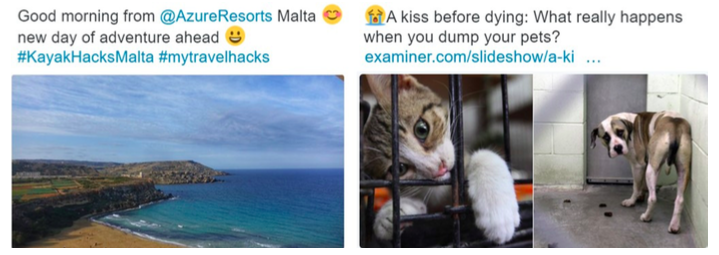
\includegraphics[width=1\columnwidth]{figs/figure1.png}
\caption{tweets中带有表情的例子,我们的模型就是在类似图中显示的文本和媒体信息上进行表情推荐。}
\label{fig:twitter}
\end{figure}


尽管问题十分的繁杂,但我们还是可以从以往的工作中理清头绪,找到一些启发: 


1)在语言模型上,以RNN(Recurrent neural network)为代表的序列模型在各个层面上都取得了很好的效果。在自然语言处理(Natural Language Processing)上,RNN和其变形LSTM(long short term memory)的效果都得到了很好的验证,尤其在机器翻译\cite{cho2014learning}和序列生成\cite{zaremba2014recurrent}这两个经典任务上。与本文工作相关的模型我们会在第二章节叙述。

2)在多模态的混合模型上,谷歌\cite{cao2014cross}通过LSTM和CNN将文本和图片的信息有效结合并在情感分析上得到了很好的效果。\cite{clinchant2011semantic}提出了cross-modality consistent regression(CCR)模型,能够有效的将文本和图片在同一连续空间中有效学习并获得特征。\cite{yang2013user}则进一步的将文本、图片之外的社会信息考虑进来得到了一个用户级别的情感预测模型。


对于表情来说,之前的工作基本都是将表情认为是情感分类的一种标签来进行处理,但这是有很大问题的。正如我们之前提到的,表情中不仅集成了情绪的成分,同时也有着丰富的语义信息,甚至比个体词汇还要丰富。我们的模型正是基于这个现象,将表情作为语言的一部分来进行处理。基于此,我们提出一个集成文本语义信息和图片视觉信息的LSTM模型来解决表情推荐的任务,能同时预测表情的位置和品种;构建了一个可用于表情推荐任务的大规模数据集合,其中包含了英文和中文两种语言以及对应的其他媒体信息(如对应图片)。问题具体的描述与定义以及模型将在第三章节叙述,而实验部分和结论将在第四和第五章节叙述。


\section{相关工作}
	\subsection{Emoticon in Social Networks}

	\cite{miller2016blissfully}表明,表情在交互平台上的普遍性,并且提出了在不同的平台上表情所给人的感觉和意义是有偏差的,甚至在某种程度上给交互带来了混乱。论文主要在表情所表达的情感等级上进行了实验,通过不同平台之间表情在情绪上的差异来进行对比。结论非常明显的指出,跨平台之间的相同意义表情给人的信号和人对其的观感是存在很大差异的。由此可以得到两个结论,一是表情蕴含丰富的语义和情绪信息;二是表情的具体内涵和其存在的上下文有直接联系而不单单是其本身定义的含义,因而根据文本和其它媒体信息对表情进行预测和推荐具有一定的可行性。

	\subsection{Distributed Representations of Sentences, Documents and Words}

		给定一个大规模的文本语料,我们可以无监督的从语料中学习到所有词的向量表示,并且这些词向量将是所有文本工作的重要基础。同样的原理,我们还可以对整个句子乃至整个文档进行向量表示。这套算法的核心思想在于定义了一套无监督的训练任务,任务就是最大可能的通过某一段间断的上下文来预测其中的词语,或者反之亦然\cite{mikolov2013distributed},并根据这个任务的正反两个方向分别构建了Continuous bag-of-words (CBOW) 模型\cite{mikolov2013efficient} 和 Skip-Gram \cite{mikolov2013linguistic} 模型,如图 \ref{fig:cbowskip}所示。基于这两种不同的无监督训练,我们可以学到非常有效的词向量表示。相比以往通过矩阵分解的词向量表示,这套无监督的学习方式可以同时集成训练语料中语法和语义的丰富特征。在以往的工作中,在文本处理的神经网络中,使用这种向量作为预处理阶段的向量初始化会极大的加快收敛速度并提高准确性\cite{erhan2010does}。
		
		\begin{figure}[htb]
				\centering
				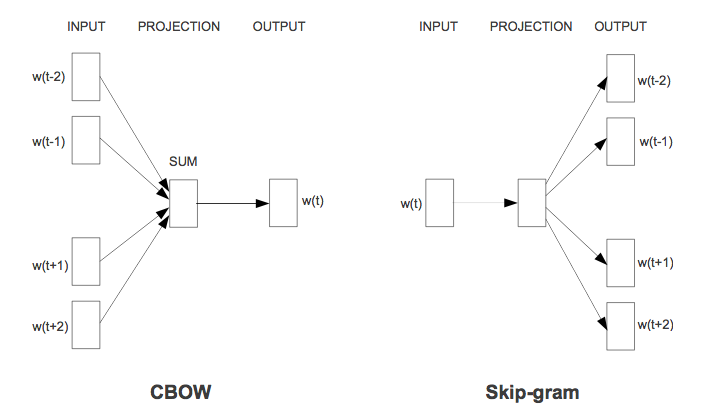
\includegraphics[height=6cm]{figs/7.png}
				\caption{CBOW and Skip-Gram}
				\label{fig:cbowskip}
		\end{figure}

		虽然CBOW和Skip-Gram的机理是完全相反的,但本质上是等价的。训练方式上有些差别,Skip的准确率会高出一些,但是训练效率上CBOW要快速很多,在语料内容很大的情况下,两者的差距影响不大。在我们的工作中,我们采取了CBOW来构建基础的文本内容的表示。


	\subsection{Sequence to Sequence Learning with Neural Networks}
		谷歌\cite{sutskever2014sequence}提出了序列到序列的神经网络模型并影响到之后的很多工作,这篇论文较早地探索了序列到序列的神经网络模型在自然语言处理任务上的效果,并在机器翻译上获得了提升。后续的研究者在其基础上进行了更广泛的应用,无论是自动文本摘要,对话机器人,问答系统等等。其主要思想如图 \ref{fig:seq2seq}所示,以机器翻译的原文结束符为中界,左边是Encoder部分,右边是Decoder部分,两边都采用LSTM模型,Decoder本质上是一个递归神经网络(RNN)语言模型,不同的是在生成词的时候依赖于Encoder的最后一个隐层向量。
			\begin{figure}[htb]
				\centering
				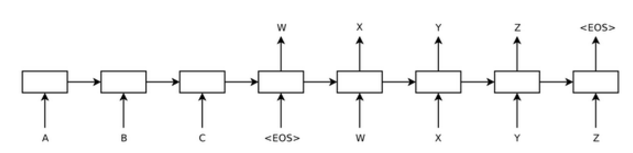
\includegraphics[width=1\columnwidth]{figs/10.png}
				\caption{序列模型}
				\label{fig:seq2seq}
			\end{figure}
		模型的优化目标就是Decoder输出部分与实际部分尽可能相似。序列模型在很多任务上有着使用情景,在我们的任务中,对表情的位置预测实际就是一个序列到序列的问题,输入文本的每个词汇后均有可能放置表情,我们的工作某种程度上等价于输入文本到位置概率分布的翻译过程。详细的一些和序列模型相关的工作将在下一部分阐述。

	\subsection{Maching Reading and Comprehension}
		机器阅读理解是最近自然语言处理里比较重要的一个环节,首先让机器学会阅读理解是一件十分重要的事情,理解文本对表情的推荐有重要意义;其次在机器阅读理解的任务中,序列到序列,端到端以及加入注意力特性的模型都被研究过;另一方面机器阅读理解的任务模式和本文中的任务有很大的相似性,对我们问题的解决具有很强的借鉴意义。用来衡量机器阅读理解效果的任务就是简单的完形填空(cloze-style),问题可以表述为一个三元组(d, q, a),这里d是指原文document,q是指问题query或者question,a是answer,即问题的答案。这个答案是来自一个固定大小的词汇表A中的一个词。机器阅读理解要解决的问题就变成了:给定一个document和query构成的pair对(d, q),从A中找到最合适的答案a。(d, q)构成的pair和我们任务中的文本和图片对应,答案集合A与表情集合对应,从这个角度来看,两者有着很强的关联性。直观上来讲,用神经网络来处理阅读理解的问题实质上是一个多分类的问题,通过构造一些上下文的表示,来预测词表中每个单词的概率,概率最大的那个就是所谓的答案,近来的研究主要也集中在如何有效的构建这个分类器上。

		\subsubsection{Deep LSTM Reader}
		在\cite{hermann2015teaching}中提到了一个简单的序列模型,如图 \ref{fig:DeepLSTMReader}所示。主要的思路就是不严格区分问题(query)和文本(document),将两者拼接作为分类器的输入,通过两层LSTM的编码得到query和document的混合特征,即是LSTM最后的隐层向量,而这个隐层向量可以进行答案的选取。
			\begin{figure}[htb]
			\centering
			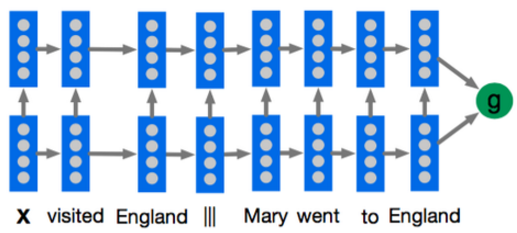
\includegraphics[width=0.6\columnwidth]{figs/1.png}
			\caption{Deep LSTM Reader}
			\label{fig:DeepLSTMReader}
			\end{figure}

		\subsubsection{Attentive Reader}
		但简单的Deep LSTM Reader模型对document和query的利用还是偏低的,实际上并不是所有的词汇都是对我们理解文意有作用,在\cite{hermann2015teaching}还提到了一个加入注意力特征的模型Attentive Reader,如图 \ref{fig:AttentiveReader}。这个模型将document和query分开表示,并且对于document和query都用双向的LSTM进行编码。双向编码的意义在于,编码内部不仅蕴含着前文的信息,后文的影响也被考虑进去了,以往按照阅读顺序进行训练的模型是没法做到这样双向的上下文关联的。LSTM后将两个方向上的最后的隐层向量作为query的特征的表示,而对于document部分则将每个词汇的前向后向隐层向量合并加权平均得到表示,这里的权重就是所谓的注意力(attention)性质,用以对词汇进行价值的区分,权重越大表示对回答的影响越重要,之后合并特征向量进行预测。
			\begin{figure}[htb]
			\centering
			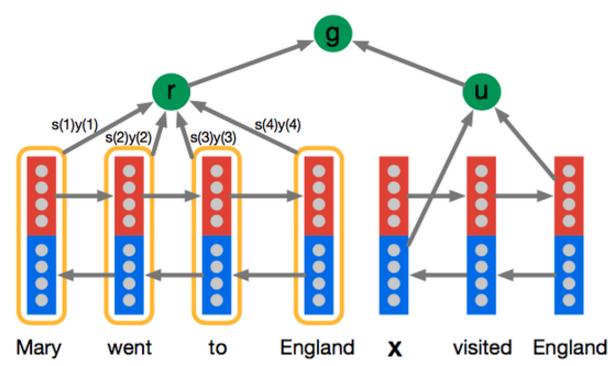
\includegraphics[width=0.6\columnwidth]{figs/2.png}
			\caption{Attentive Reader}
			\label{fig:AttentiveReader}
			\end{figure}

		\subsubsection{Impatient Reader}
		这个模型在Attentive Reader模型的基础上更细了一步,认为每个query中的词汇都和document中的词汇有关联。所以将query中的每个词汇都和document进行一次结合来提取特征,如图 \ref{fig:ImpatientReader}所示。直观上来理解,这个过程类似于人类不断的看query再读document,每读到query的一个词汇就去联系document中与之对应的词汇,从而得到答案。这个模型虽然更加复杂一些,但效果不见得很好,从人的实际体验来说是不可能读query中的每一个词之后,就去读一遍原文,这样效率太低了,而且原文很长的话,网络的记忆负担会急剧增大,违背了LSTM重点记忆的出发点,导致最后记忆效果的下降。
			\begin{figure}[htb]
			\centering
			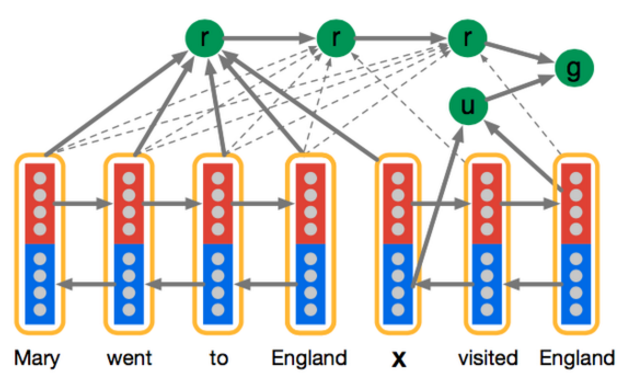
\includegraphics[width=0.6\columnwidth]{figs/3.png}
			\caption{Impatient Reader}
			\label{fig:ImpatientReader}
			\end{figure}

		\subsubsection{Attention Sum Reader}
		刻意复杂的模型不一定一定效果明显,IBM\cite{kadlec2016text}提出了一套简单有效的Attention Sum Reader模型,并对之后的工作起到了很大影响。其模型如图 \ref{fig:AttentionSumReader}所示。模型分为五层,第一层将document和query的词汇分别映射为词向量,第二层使用双向的GRU来对document和query进行编码,从而得到各自document内容在连续空间的表示,其中document中每个词汇就用GRU前向后向的隐层向量表示,query则用GRU两个两个方向的最后的隐层向量表示。每个document中词汇的双向GRU输出与query的输出作点积并归一化后得到每个词的权重(词汇与query的相关程度)。与Attentive Reader相比Impatient Reader,Attention Sum Reader的attention的机制更为合理。同样从实际场景出发,我们可以读query之后带着query的提示去读原文从而最终获取答案,Attention Sum Reader的模型很符合这一机理。
			\begin{figure}[htb]
			\centering
			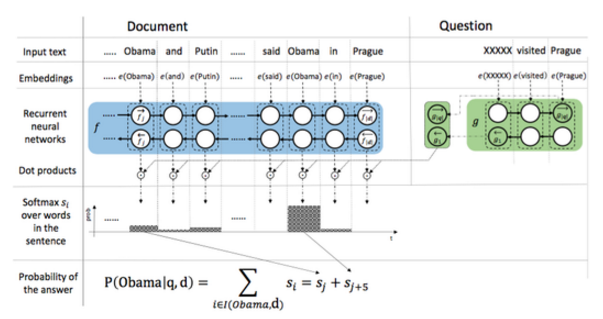
\includegraphics[width=0.6\columnwidth]{figs/4.png}
			\caption{Attention Sum Reader}
			\label{fig:AttentionSumReader}
			\end{figure}

		\subsubsection{Gate Attention Reader}
		Gate Attention Reader\cite{dhingra2016gated}是Attention Sum Reader的一个多轮迭代强化版本,每轮迭代中基本操作方案和Gate Attention Reader是一致的,如图 \ref{fig:GateAttentionReader}。模型将document和query通过一个词汇查询层,使得每个词都表示成一个低维向量。之后将document中的词向量通过一个双向GRU,将两个方向的state做拼接获得该词的新表示。同时也将query通过一个双向GRU,用两个方向上的最后的隐层向量作为query的向量表示。之后将GRU输出的新的词汇表示与query的新表示逐元素相乘得到下一个GRU层的输入。在这样的操作迭代若干轮之后送进分类器从而进行结果的预测。实验结果表明,在一定轮数迭代之后,原本的模型效果得到了不小的提升,这种类似多次带着query读document的实现机理能有效将单层结构拓展到高层。
			\begin{figure}[htb]
			\centering
			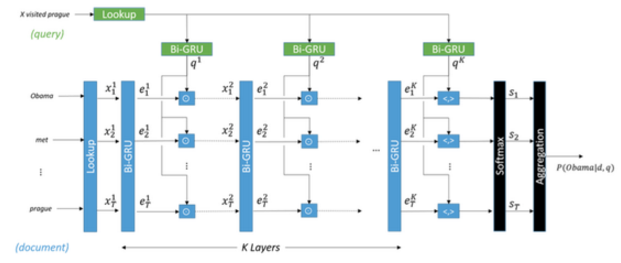
\includegraphics[width=0.6\columnwidth]{figs/5.png}
			\caption{Gate Attention Reader}
			\label{fig:GateAttentionReader}
			\end{figure}

		\subsubsection{Iterative Alternating Attention}
		Iterative Alternating Attention \cite{sordoni2016iterative}是Bengio组的新作,主要的不同之处在于,将attention机制也交给一个神经网络去进行。如图 \ref{fig:IterativeAlternatingAttention}所示,query和document编码之后传入中间的RNN进行反复迭代,中间RNN最后的隐层向量用来进行结果的预测。虽然模型相对复杂,但效果与Gate Attention Reader伯仲之间,并没有体现太多attention上的优越性,不过这种基于数据驱动的attention机制是值得借鉴的。
			\begin{figure}[htb]
			\centering
			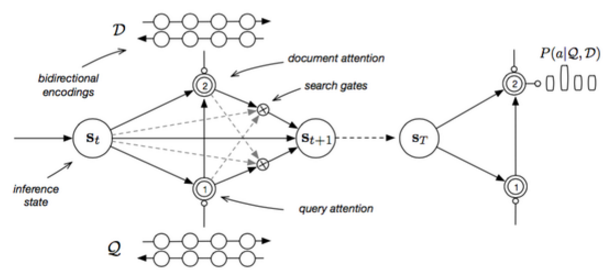
\includegraphics[width=0.6\columnwidth]{figs/6.png}
			\caption{Iterative Alternating Attention}
			\label{fig:IterativeAlternatingAttention}
			\end{figure}

	\subsection{Mutiple Model Joint Learning}

		谷歌\cite{vinyals2015show}在2015年在情感分析上提出了一个多模态的混合模型,将文本和图片有机的结合在一起。如图 \ref{fig:multisample1}所示,模型的基本框架是用卷积神经网络(CNN)训练图片特征和递归神经网络的变种(LSTM)训练文本特征,然后结合共同进行文本和图片的情感预测。
		因为局部块状特征的采样,CNN很适合处理图片;而语言因为其序列的特性,LSTM能很好的提取文本的特征。这个混合模型框架针对不同的输入采用不同的特征采样器,相比于统一模型处理多模态能够更好的保留图片与文字各自的特点。
			\begin{figure}[htb]
				\centering
				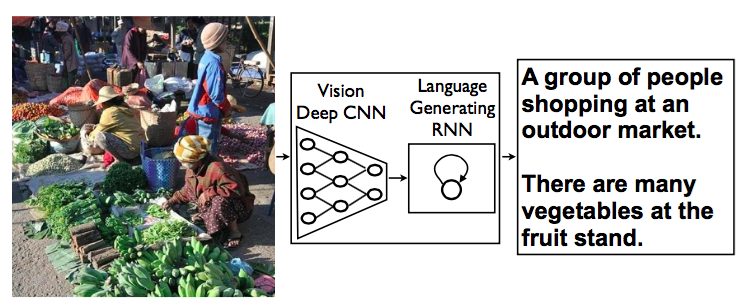
\includegraphics[width=0.6\columnwidth]{figs/8.png}
				\caption{图片与文本的结合总体框架}
				\label{fig:multisample1}
			\end{figure}
		
		而在具体结合过程中,如图 \ref{fig:multisample2}所示,CNN输出的图片特征被作为语义输入和文本一起输入到LSTM中进行训练。图片和文本本身在不同的空间,如果采用一个映射矩阵将两者映射到统一空间在效率上会有很大问题;如果将两者向量拼接起来进行分类,这种混合方式就比较简单。此模型采用了Joint Learning的方式,将CNN的图片特征放到语义空间中,和语义训练模型一起进行反馈,从而减少了映射的模型复杂度又很好的将两者特征融合在一起。
			
			\begin{figure}[htb]
			\centering
			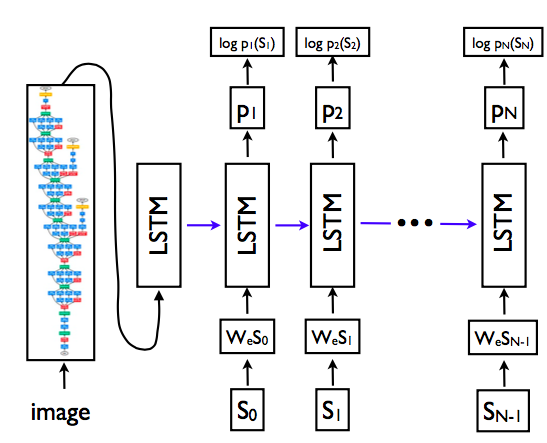
\includegraphics[width=0.6\columnwidth]{figs/9.png}
			\caption{具体的结合模型}
			\label{fig:multisample2}
			\end{figure}

		\cite{you2016cross}在传统模型上也提出了一套混合训练方案,也具有借鉴意义。

\section{模型}


\subsection{Recurrent Neural Networks (RNN)}

在人工智能中我们总是希望通过模型来表现人类的一些行为,无论是在音频、图像还是文字上。我们考虑人类的认知行为,虽然现在无法定量的进行分析,但还是可以定性的进行一些分析。在整个过程中不难发现,这样一个复杂的行为过程中的每一步都不是独立的,并且存在时序上的影响关系,换句话说,我们在思考一个大问题的各个子环节时并不是从一片空白开始的,而是在过去一定时间范围内的信息基础上进行的。比如在我们任务中的文字理解上,在阅读某一篇文章的时候,我们都是基于自己已经拥有的对先前所见词的理解来推断当前词的真实含义,虽然我们的记忆具有遗忘性,但我们不会将所有的东西都全部丢弃,然后每每用空白的大脑再进行思考。传统的模型,无论是普通的线性模型还是神经网络都不能很好的拟合这样的一种特性,在时序这一特性上存在缺失。


			\begin{figure}[htb]
			\centering
			\includegraphics[width=0.6\columnwidth]{figs/RNN.png}
			\caption{Recurrent Neural Networks (RNN)}
			\label{fig:RNN}
			\end{figure}

Recurrent Neural Networks (RNN)将时序状态机引入到神经网络中,通过时序状态机的循环工作使得信息的持久化成为可能,时序性在模型中得到了体系。在上面的示例图图 \ref{fig:RNN}中,一个RNN的神经元模块通过读取输入$\textbf{x}_i$和上一轮的隐层向量$\textbf{h}_{i-1}$,在经过线性变换和激活函数后输出当前这一轮的隐层向量$\textbf{h}_i$,神经元的内部函数为:
$$\textbf{h}_i = \tanh(\textbf{W}\cdot[\textbf{h}_{i-1},\textbf{x}_i] + \textbf{b})$$
直观上来理解,时序状态机通过不断传递隐层的状态来实现信息的延续,以往的模型神经元的输出只与输入相关,而在RNN中,输出不仅与输入相关而且与时序在前的网络状态相关。整个的网络运行机制变的复杂了许多,但实际上理解起来却更加自然,尤其是我们将整个RNN展开并尝试用阅读这样的行为方式去类比,如图 \ref{fig:RNN1},阅读的过程就是以词为单位的序列输入,对每一个词的理解依赖于其前文的铺垫。


			\begin{figure}[htb]
			\centering
			\includegraphics[width=0.8\columnwidth]{figs/RNN1.png}
			\caption{Recurrent Neural Networks (RNN)}
			\label{fig:RNN1}
			\end{figure}


在过去的几年中,RNN也已经被广泛应用了,包括语音识别,语言建模,翻译,图片描述等问题上。链式的特征揭示了RNN本质上是与序列和列表相关的,对于这类数据的最自然的神经网络架构,因而在语言的相关任务上效果十分明显。我们也采用这样的网络来开展我们的任务,但根据我们的实际需要,我们使用了Long-Short Term Memory (LSTM)这个RNN的变形来进行工作。LSTM是一种特别的RNN,因为其在“记忆”上的独特特性,该模型比标准的RNN在很多任务上要表现得更好,具体的细节我们将在之后的模型章节介绍。


\subsection{Long-Short Term Memory (LSTM)}

RNN的关键特性之一就是他们可以用来连接先前的信息到当前的任务上,也就是时序性质,例如之前我们提到的通过上文的信息来辅助理解当前的词语。但实际上,出于解决这个问题而被构建出来的RNN在解决这个问题时还是有不少问题存在,一个最明显的问题就是长效记忆,或者说是长期依赖问题。

还是用语言理解来举例子,如果我们现在让计算机来进行完形填空的任务,对于一些短句,如“The capital of China is Beijing”,“capital”和“China”构成的前文可以预测最后的结果“Beijing”,在这样的场景中,相关的信息和预测的词位置之间的间隔是非常小的,RNN可以很不错地学会使用先前的信息。

但是同样会有一些更加复杂的长句,尤其是逻辑链很长的情景下,诸如我们试着去预测“William Shakespeare wrote Hamlet ... He is a great writer”,在这种情况下,前文的相关信息“William Shakespeare wrote Hamlet”和当前预测位置“writer”之间的间隔会变得相当的大,RNN的前文信息传递过程中每个词的占比权重实际上是不均等的,后出现的词远比先出现的词影响能力要来的强烈。当这个依赖间隔不断增大时,前文的有效信息会被逐渐冲淡,以至于RNN丧失学习到连接如此远的信息的能力。

从模型的理论性能上来讲,长效的记忆属性,也就是长期依赖,RNN也是可以处理的,一定会存在一个特定的参数能够使得这样的情况得到很好的拟合。但这在实际操作中是难以做到的,或者说根本无法做到,毕竟我们无法仔细挑选整个网络浩繁的各个参数。所以在模型的实际训练过程中,这样的“完美”参数是绝对无法成功学习到的。在\cite{Bengio1994Learning}中,这个问题得到了深入的研究,他们发现一些使训练 RNN 变得非常困难的相当根本的原因。


为了解决这个问题,Long Short Term Memory (LSTM)由\cite{Hochreiter1997Long}提出,并在近期被进行了改良和推广。在很多问题,LSTM 都取得相当巨大的成功,并得到了广泛的使用。如图 \ref{fig:LSTM},LSTM的关键就是细胞状态(cell),即为在图上方贯穿运行的水平线。细胞状态类似于传送带,直接在整个链上运行,只有一些少量的线性交互,信息在上面流传保持不变会很容易。LSTM同时 通过精心设计的门(gate)结构来去除或者增加信息到细胞状态的能力。门是一种让信息选择式通过的方法,他们包含一个sigmoid神经网络层和一个各位相乘的向量操作。sigmoid函数的特性就是输出0到1之间的数值,在LSTM中被用来描述每个部分有多少量可以通过,0代表无通过,1代表全通过。LSTM通过三个门来保护和控制细胞状态和这个网络的运行。



		\begin{figure}[htb]
		\centering
		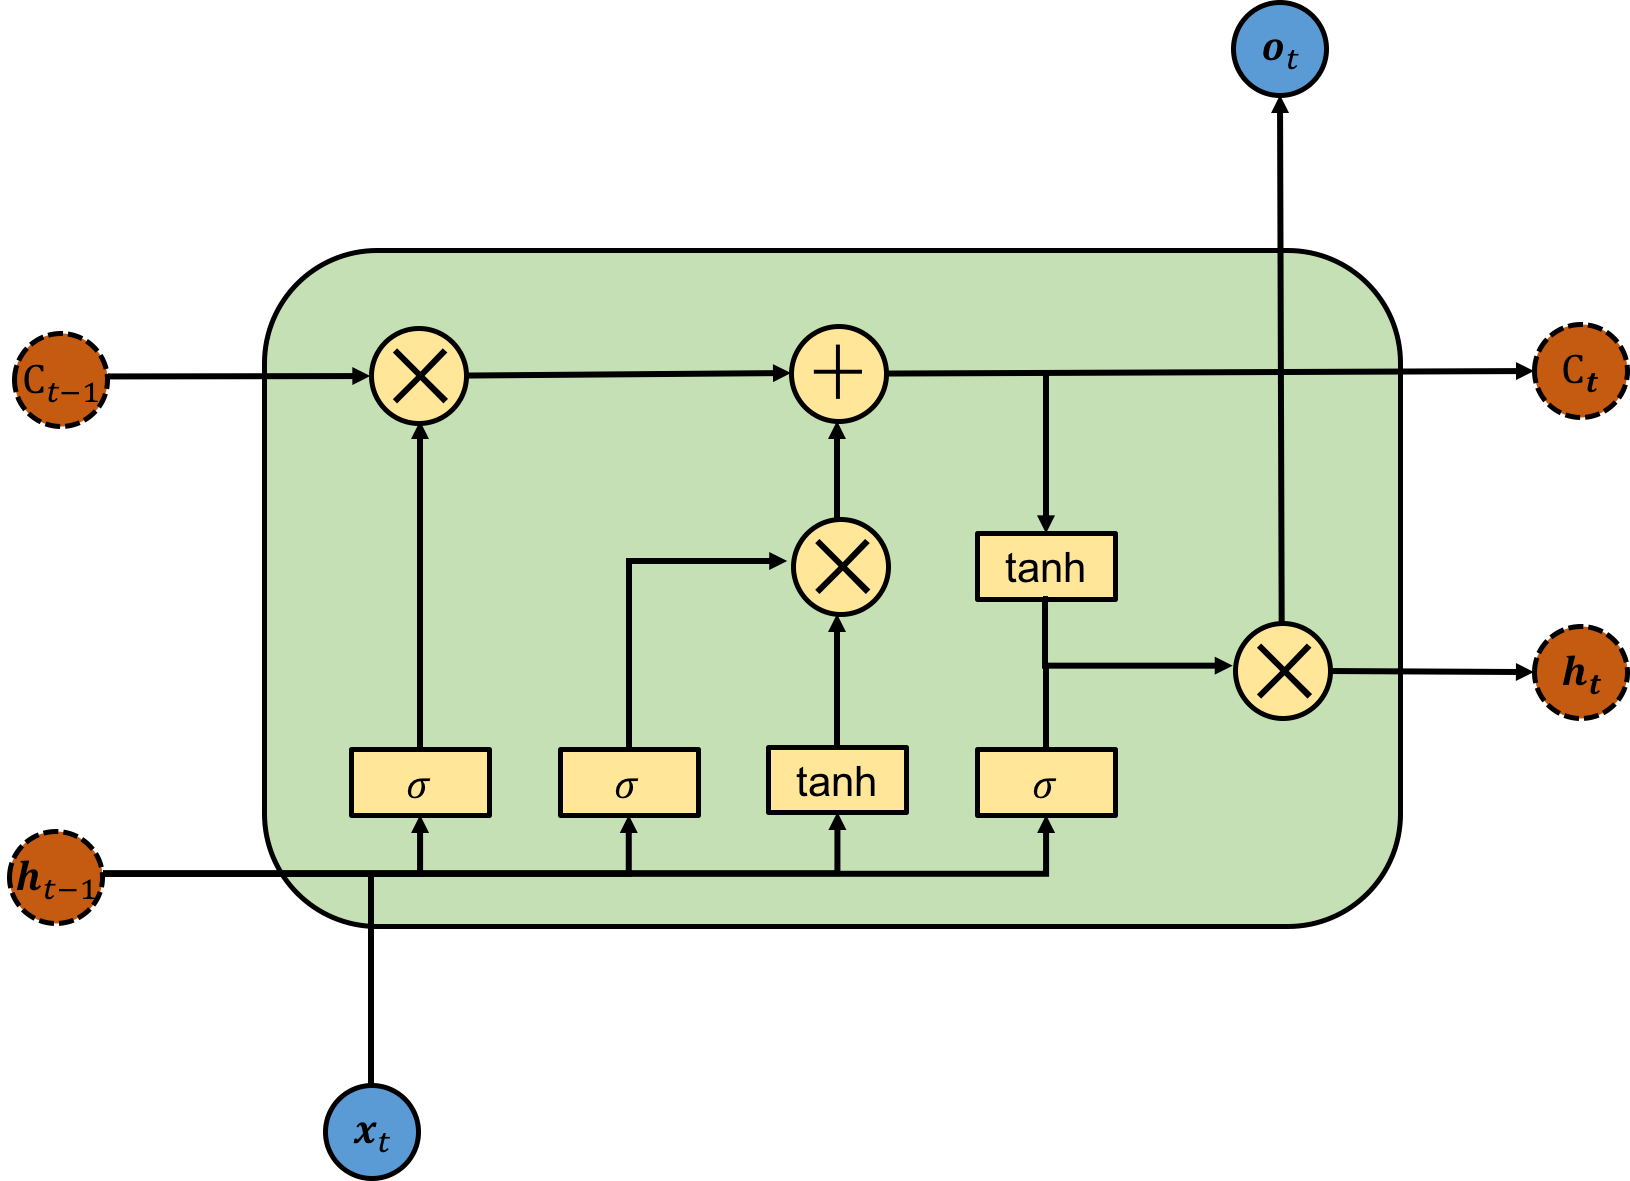
\includegraphics[width=0.8\columnwidth]{figs/LSTM.png}
		\caption{Long-Short Term Memory (LSTM)}
		\label{fig:LSTM}
		\end{figure}


LSTM中的第一步是决定会从细胞状态中丢弃什么信息。这个决定通过一个称为忘记门层的sigmoid函数完成。该门会读取$\textbf{h}_{t-1}$和$\textbf{x}_t$,输出一个在0到1之间的数值给每个在细胞状态$\textbf{C}_{t-1}$中的特征进行过滤,1表示完全保留,0表示完全舍弃。

$$\textbf{f}_t = \sigma(\textbf{W}_f \cdot [\textbf{h}_{t-1}, \textbf{x}_t] + \textbf{b}_f)$$

决定丢弃信息的之后一步是确定什么样的新信息被存放在细胞状态中。这里包含两个部分。一个称为输入门层的sigmoid层,决定什么值我们将要更新。然后,一个激活函数tanh的激活层用来创建一个新的细胞状态候选值向量$\tilde{\textbf{C}}_t$,并将其加入到状态中。

$$\textbf{i}_t = \sigma(\textbf{W}_i \cdot [\textbf{h}_{t-1}, \textbf{x}_t] + \textbf{b}_i)$$
$$\tilde{\textbf{C}}_t = \sigma(\textbf{W}_C \cdot [\textbf{h}_{t-1}, \textbf{x}_t] + \textbf{b}_C)$$

在获取新的细胞状态候选值向量$\tilde{\textbf{C}}_t$后,LSTM将细胞状态$\textbf{C}_{t-1}$更新为$C_t$。新的细胞状态$C_t$由旧状态$\textbf{C}_{t-1}$通过忘记门层$\textbf{f}_t$,丢弃掉我们确定需要丢弃的信息,和新的细胞状态候选值向量$\tilde{\textbf{C}}_t$通过输入门层$\textbf{i}_t$过滤之后相加而成,即

$$\textbf{C}_t = \textbf{f}_t * \textbf{C}_{t-1} + \textbf{i}_t * \tilde{\textbf{C}}_t$$


最终,我们需要确定输出什么值。这个输出将会基于我们的细胞状态,但是也是一个过滤后的版本。首先,我们运行一个sigmoid层来确定细胞状态的哪个部分将输出出去。接着,我们把细胞状态通过tanh进行激活并将它和sigmoid门的输出相乘,最终我们仅仅会输出我们确定输出的那部分。

$$ \textbf{o}_t = \sigma (\textbf{W}_o \cdot [\textbf{h}_{t-1},\textbf{x}_t]+\textbf{b}_o) $$
$$ \textbf{h}_t = \textbf{o}_t * tanh(\textbf{C}_t)$$

我们采用了LSTM作为我们基础的训练模型来解决我们的任务。

\subsection{Gated Recurrent Unit (GRU)}

我们的任务需要很好的对语义进行理解,一个词不仅需要考虑前文的信息,且对下文也有着深刻的影响,所以我们需要一种同时考虑到前后文的模型的词向量生成模型,这里我们采用了双向迭代门单元(Bidirectional Gated Recurrent Unit)的模型来进行。Gated Recurrent Unit (GRU)是由\cite{cho2014learning}提出的LSTM的变种。GRU的一个显著特点在于模型本身将忘记门和输入门合成了一个单一的更新门。对应的,模型还混合了细胞状态和隐藏状态,使得中间传递的又和RNN类似,只存在一个隐层传递向量,整体的模型如图 \ref{GRU}所示,比标准的LSTM模型要简单。

		\begin{figure}[htb]
		\centering
		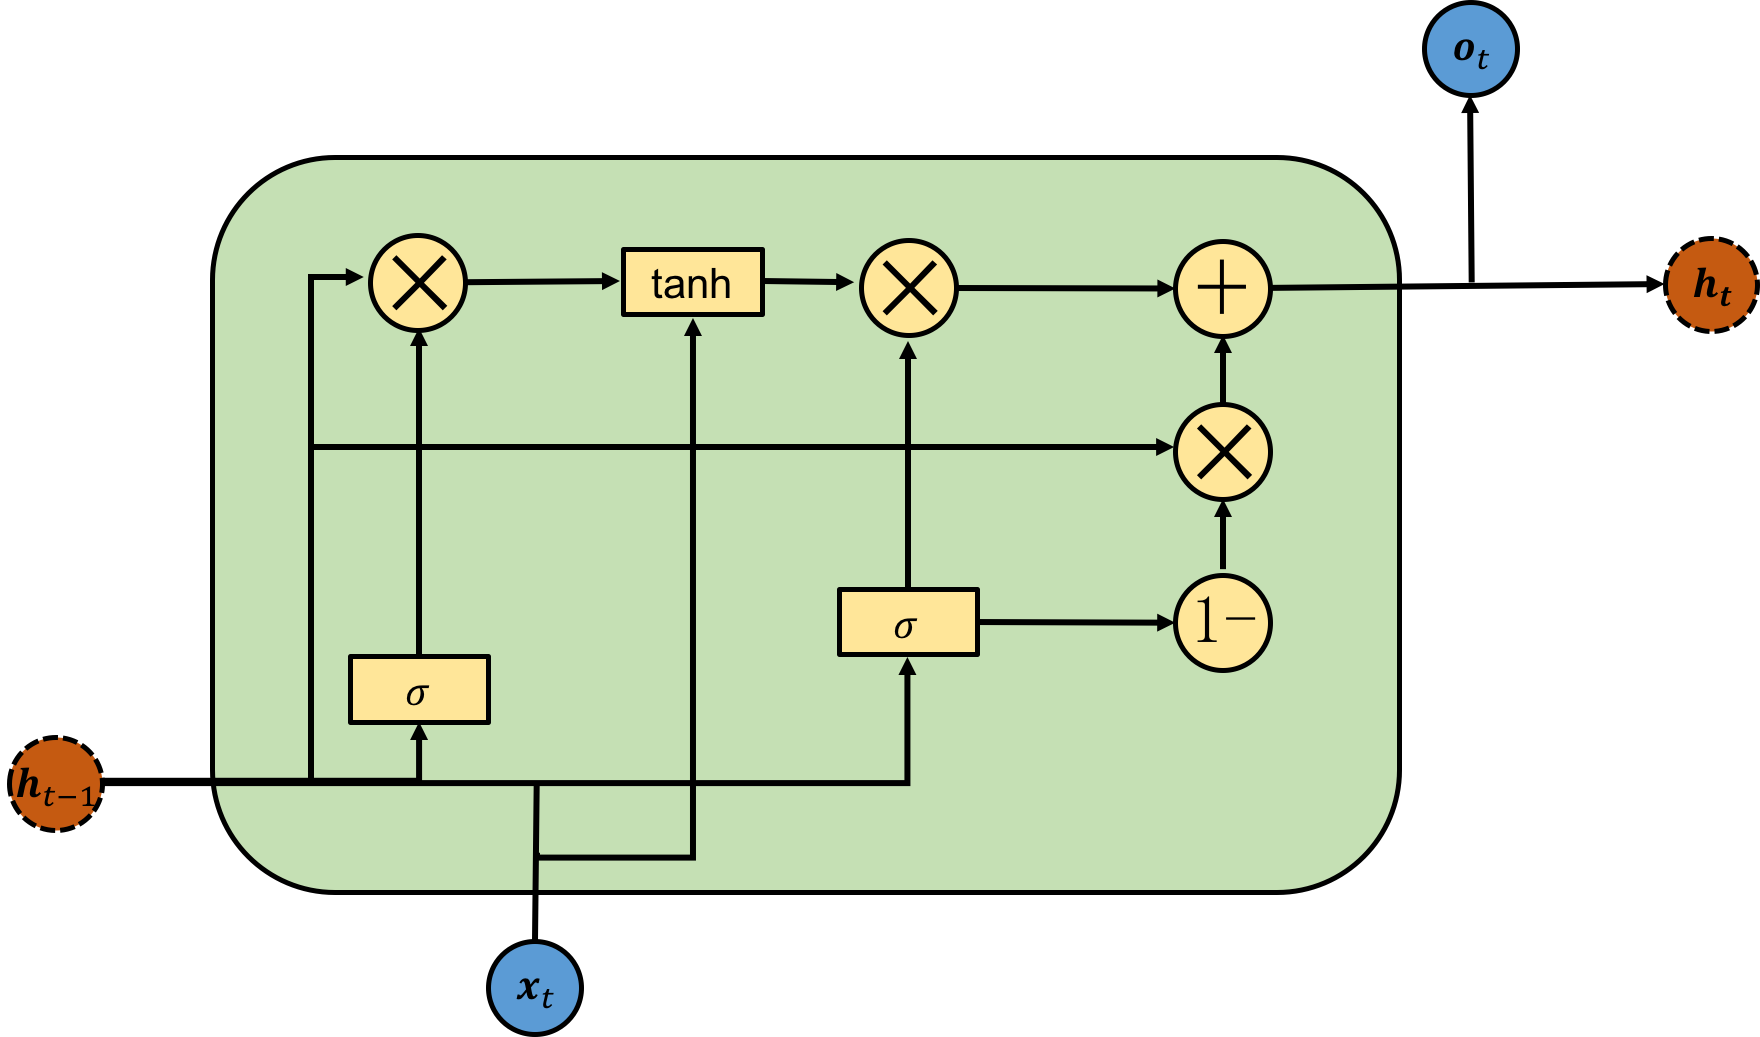
\includegraphics[width=0.9\columnwidth]{figs/GRU.png}
		\caption{Gated Recurrent Unit (GRU)}
		\label{fig:GRU}
		\end{figure}

对于输入的隐层向量$\textbf{h}_{t-1}$和输入向量$\textbf{x}_t$,计算得到输入隐层向量的过滤门$\textbf{r}_t$,
$$\textbf{r}_t = \sigma(\textbf{W}_r \cdot [\textbf{h}_{t-1},\textbf{x}_t])$$

通过过滤门后的隐层向量$\textbf{h}_{t-1}$和输入向量$\textbf{x}_t$,在线性变换和激活之后得到隐层向量的新候选向量$\tilde{\textbf{h}_t}$,
$$\tilde{\textbf{h}_t} = \tanh(\textbf{W} \cdot [\textbf{r}_t * \textbf{h}_{t-1},\textbf{x}_t])$$

输出向量和传递的隐层向量合为一体,并且有输入的隐层向量$\textbf{h}_{t-1}$和新候选向量$\tilde{\textbf{h}_t}$按比例合成,合成的比例也是通过一级过滤门来实现的,

过滤门$\textbf{z}_t$,

$$\textbf{z}_t = \sigma(\textbf{W}_z \cdot [\textbf{h}_{t-1},\textbf{x}_t])$$

合成$\textbf{h}_t$,

$$\textbf{h}_t = (1 - \textbf{z}_t) * \textbf{h}_{t-1} + \textbf{z}_t * \tilde{\textbf{h}}_t$$

在我们的模型中,我们采用了双向的GRU来对词进行向量化,如图 \ref{fig:bi-gru}所示。在双向GRU中,从文本序列的顺序和逆序分别进行GRU编码,每个词汇
用其顺序的输出向量$\textbf{o}^{forward}_t$和逆序的输出向量$\textbf{o}^{backward}_t$拼凑成的$\textbf{o}_t = [\textbf{o}^{forward}_t, \textbf{o}^{backward}_t]$取代其粗糙的$\textbf{x}_t$用以传入之后的工作模型,从而使得每个词的输入向量即包含前文的特征又蕴含后文的特征。

		\begin{figure}[htb]
		\centering
		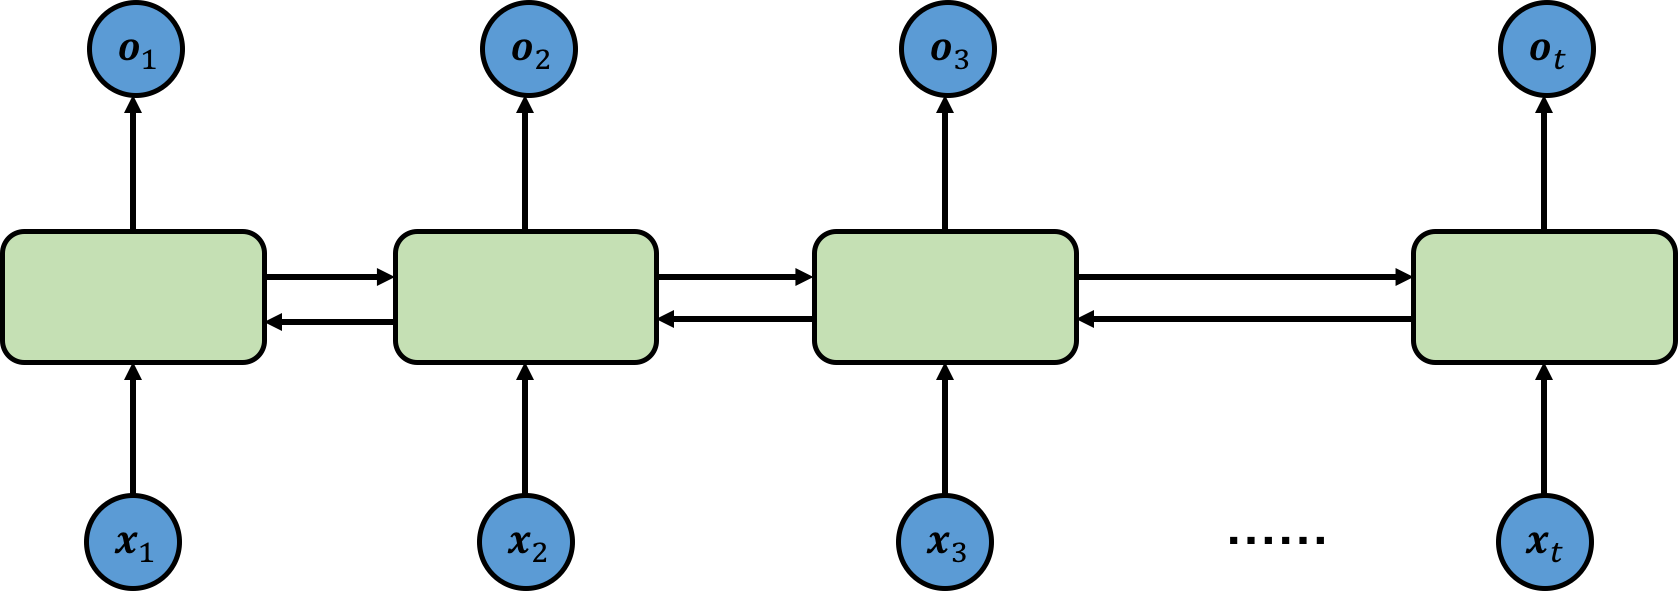
\includegraphics[width=0.8\columnwidth]{figs/bi-gru.png}
		\caption{Bidirectional Gated Recurrent Unit}
		\label{fig:bi-gru}
		\end{figure}


\subsection{Model for Emoticon Prediction}

基础的表情预测模型部分,我们直接采用LSTM来进行表情的类别和位置的预测。此外为了充分考虑到前后文的信息从而能够更好的将特征融合进预测模型中,我们在LSTM之前的词向量输入层和LSTM之间插入了一个双向GRU的词向量编码层,用以对词向量的前后文进行学习。

文本内容在经过神经网络的处理之后获得输出向量,我们对输出向量进行了池化操作得到了最后的特征,在池化后的特征基础上我们构建分类器和损失函数分别对表情的类别和位置进行预测训练。

\subsection{Joint Model}

图像信息的融合,我们采取了Joint Learning的方法,将图像的向量通过矩阵映射直接投影到文本的空间内和文本内容一起输入进神经网络的分类器中进行训练。


\section{实验}

\subsection{实验设置}

为了验证我们的模型的有效性,我们用现实存在的数据来进行验证。我们的验证采用了两种不同的任务来衡量,一个是表情的类别预测,一个是表情的位置预测。在实验对象的设置上,我们将相同的词向量和图像向量输入到不同模型中,通过比较各自的预测准确性来衡量其有效性。实验一共涉及到四个模型,分别是支持向量机(SVM)模型,逻辑回归(LR),我们的基础模型LSTM,和加入了双向GRU优化词向量之后的多层模型(GRU+LSTM)。
我们将现实中的社交平台数据按照表情的分布以十折交叉测试的方式划分训练集合和测试集合。在测试过程中,我们将表情从文本中去除,使得测试的过程接近于真实的表情插入环境,在结果的评测上我们要求预测的类别必须与去除前一致才算类别正确,位置必须与原位置一致才算位置正确,其余均为预测错误,通过测试集合的准确率来进行衡量。

\subsection{数据设置}

		我们分别在中文和英文两个最大的社交平台微博和Twitter上进行试验数据的构建,按照整体的表情分布比例来随机抽取现实社交平台上的文本和图像。中文微博和英文推特的表情比重分布统计图如图 \ref{fig:tongji}所示。我们选取了其中存在一个表情的发布状态来测试我们的模型,中文共计270041个状态,35个表情;英文共计164880个状态,35个表情。

		\begin{figure}[htb]
		\centering
		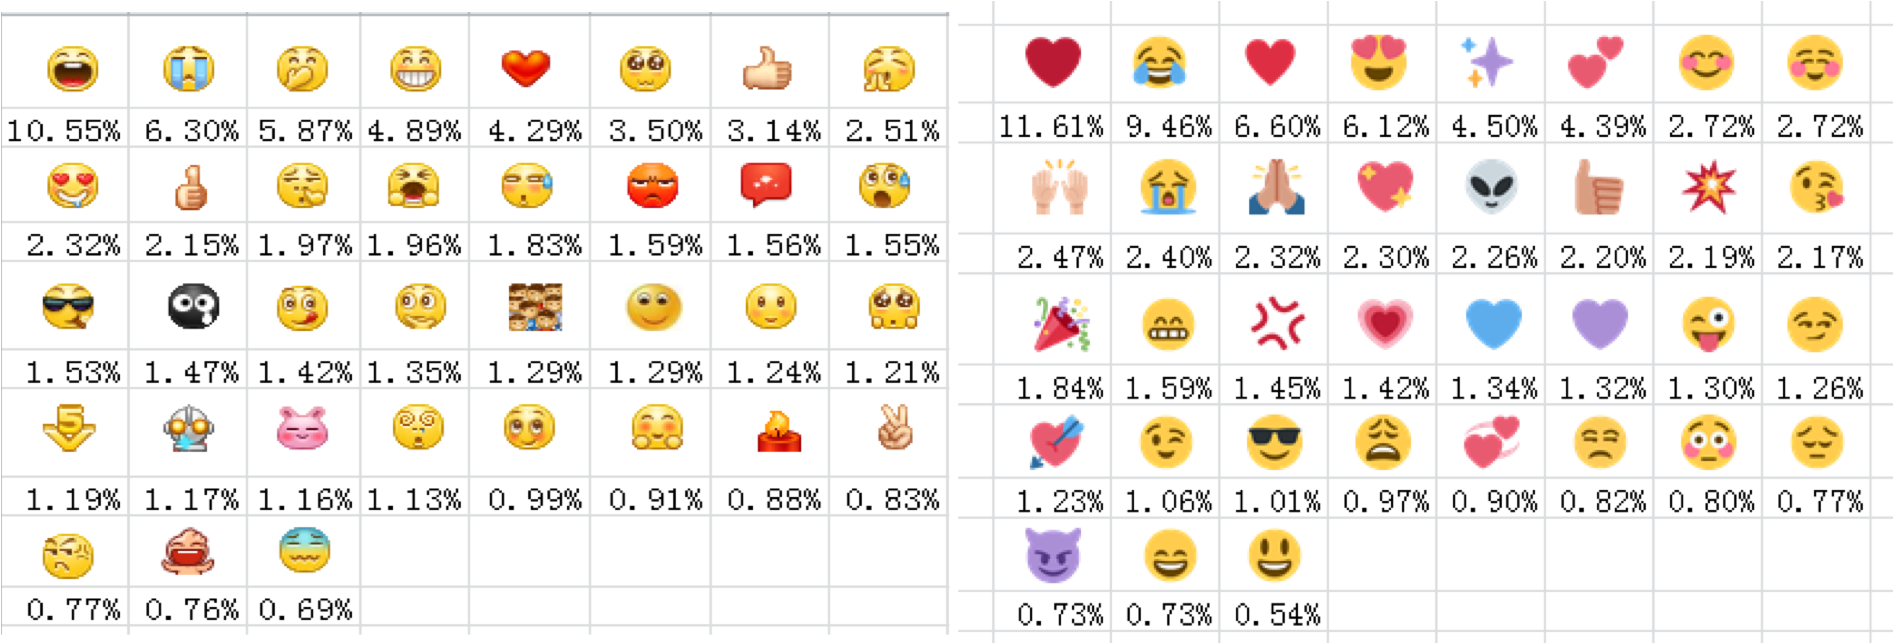
\includegraphics[width=0.8\columnwidth]{figs/fenbu.png}
		\caption{中文微博和英文推特的表情比重分布统计图}
		\label{fig:tongji}
		\end{figure}


\subsection{实验参数}

我们采用了Google的开源框架TensorFlow\footnote{https://www.tensorflow.org/}来进行神经网络的构建。在GRU和LSTM的内部单元,我们采取了2层的转换,训练的batch size为64,dropout的概率为0.5,训练轮数为20,初始词向量的维度为100。训练的过程使用了Adam优化来进行分类器到神经网络的反馈,并且一直反馈到输入的词向量层。

\subsection{实验结果}


\begin{table}[htb]
\centering
\small
\begin{tabular}{|c|c|c|c|c|c|}
\hline
Models 		& \textbf{类别} & \textbf{位置}	\\ \hline
SVM			& 0.187           & 0.572		\\ \hline
LR			& 0.183           & 0.578		\\ \hline
LSTM		& 0.220           & 0.734		\\ \hline
GRU+LSTM	& \textbf{0.235}           & \textbf{0.792}		\\ \hline
\end{tabular}
\caption{中文微博结果}
\label{tab:Weibo}
\end{table}


\begin{table}[htb]
\centering
\small
\begin{tabular}{|c|c|c|c|c|c|}
\hline
Models 		& \textbf{类别} & \textbf{位置}	\\ \hline
SVM			& 0.327           & 0.759		\\ \hline
LR			& 0.317           & 0.748		\\ \hline
LSTM		& 0.386           & 0.801		\\ \hline
GRU+LSTM	& \textbf{0.391}           & \textbf{0.823}		\\ \hline
\end{tabular}
\caption{英文推特结果}
\label{tab:Twitter}
\end{table}


\subsection{实验分析}

从结果上来看,无论在英文的环境上还是在汉语的环境上,基础模型LSTM都比常见的非深度模型支持向量机和逻辑回归模型有效的多。而在采取了双向GRU来强化词的语义提取之后,LSTM分类器的效果比基础的LSTM模型又有了显著的提升,这很好的符合了我们的预期,并验证了深度模型在此项任务上的有效性。另外从结果上来看,中文的效果和英文的效果相差很大,这也是预料之中的。相比于英文,中文需要进行分词操作,分词的准确性某种程度上会影响到算法对文本的把握;另外汉语的词语在规模还是二义性上都比英文要难处理,这也是影响中文效果的重要因素。

\subsection{实验代码}

我们开源了实验代码\footnote{https://github.com/THUCSTHanxu13/Tensorflow_Test},整个实验的数据和代码都可以从github上获得。



% \section{结论}
% ToDo




\bibliographystyle{plain}
\bibliography{report}
\end{document}
